\documentclass[a4paper]{article}

\title{Rapport AP4B}
\author{Esteban Becker}
\date{P23}

\usepackage{graphicx}
\graphicspath{ {./Diagram} }

\usepackage{graphicx}
\usepackage{listings}

\begin{document}

\maketitle

\section{Model}

\begin{figure}[h]
\centering
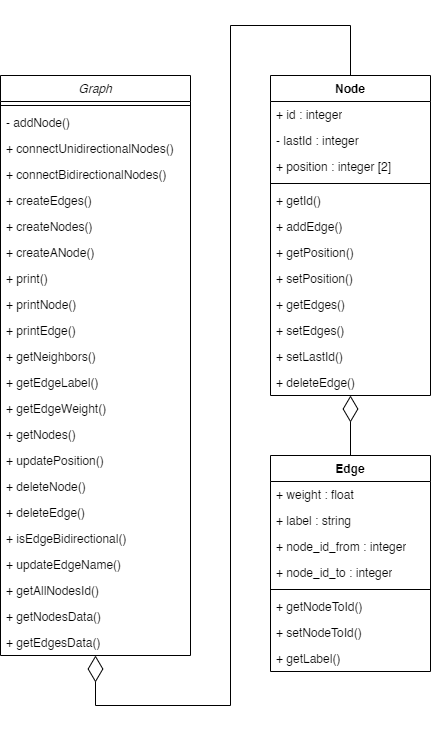
\includegraphics[width=0.7\textwidth]{report/Diagram/classGraph.png}
\caption{Diagramme de class de la class Graph}
\end{figure}

Ainsi, la class graph est composé de la class Node qui est composée de la class Edge

En code, nous l'avons implémenté avec des HashMap:

\begin{lstlisting}[language=java]
HashMap<Integer, Node> nodes;
\end{lstlisting}
\begin{lstlisting}[language=java]
HashMap<Integer, Edge> edges;
\end{lstlisting}

Nous avons choisi les HashMap car elles permettent de directement relier un id de nœud à un lui-même ou bien un id de Nœud à la liaison qu'il a avec un autre sans les numéroter de façon continue. En termes de code, nous n'avons pas à parcourir toute une liste pour trouver l'objet qui nous intéresse, il suffit d'utiliser la ligne suivant :

\begin{lstlisting}[language=java]
Node node = nodes.get(node_to_id);
\end{lstlisting}




\end{document}